% Created 2016-11-07 Mon 19:20
\documentclass{article}
\usepackage[utf8]{inputenc}
\usepackage[T1]{fontenc}
\usepackage{fixltx2e}
\usepackage{graphicx}
\usepackage{grffile}
\usepackage{longtable}
\usepackage{wrapfig}
\usepackage{rotating}
\usepackage[normalem]{ulem}
\usepackage{amsmath}
\usepackage{textcomp}
\usepackage{amssymb}
\usepackage{capt-of}
\usepackage{hyperref}
\usepackage[margin=1.0in]{geometry}
\author{Nelson Liu}
\date{\today}
\title{}
\hypersetup{
 pdfauthor={Nelson Liu},
 pdftitle={},
 pdfkeywords={},
 pdfsubject={},
 pdfcreator={Emacs 24.5.1 (Org mode 8.3.4)}, 
 pdflang={English}}
\begin{document}

\tableofcontents

\section{Naive Bayes}
\label{sec:orgheadline5}
\subsection{1. Overarching Goals}
\label{sec:orgheadline1}
\begin{itemize}
\item We want to assign each \(\bar{x} \in X\) to its correct class \(C_k\), \(k \in
  {1,...,K}\)
\item We ask: \textbf{Given} \(\bar{x} \in X\), what is its most \textbf{probable class} \(C_k\)?
\end{itemize}
\subsection{Understanding Conditional Probability}
\label{sec:orgheadline2}
\begin{itemize}
\item Sample space (\(\Omega\)) contains events whose probability of occurring is proportional to
its area w.r.t the sample space
\item In a fair coin flip, \(\mathbb{P}(heads) = \mathbb{P}(H) = \mathbb{P}(tails) = \mathbb{P}(T) = 0.5\)
\item Say we have the events \(H\), \(T\), and \(T\), where \(H\) is the event that Hillary
Clinton is elected president, \(T\) is the probability that Trump is, and \(N\) is
the probability that a nuclear winter occurs during the next presidency.
\item see figure one
\item If we want to talk about the probability of a nuclear winter happening
(\(\mathbb{P}(N)\)) given that Donald Trump is elected president
(\(\mathbb{P}(T)\)), we express it as \(\mathbb{P}(N|T)\).
\begin{itemize}
\item \(\mathbb{P}(N|T)\) is read as "probability of a nuclear winter given that Trump is
elected"
\end{itemize}
\item \(\mathbb{P}(N|T) = \frac{\mathbb{P}(N \cap T)}{\mathbb{P}(T)}\).
\begin{itemize}
\item Note that the probability of event \(T\) occurring is in the denominator,
think of this as the new sample space that has been reduced.
\item We then find the probability of \(\mathbb{P}(N \cap T)\) over this new, reduced sample
space. This is equivalent to \(\mathbb{P}(N|T) = \frac{\mathbb{P}(N \cap T)}{\mathbb{P}(T)}\).
\item see figure 2
\end{itemize}
\end{itemize}
\subsection{Bayes' Theorem}
\label{sec:orgheadline3}
\begin{itemize}
\item We can represent the entire sample space \(\Omega\) in terms of conditional
probabilities.
\item see figure 3
\item As a reminder: we want to assign each \(\bar{x} \in X\) to its correct class \(C_k\), \(k \in
  {1,...,K}\)
\item We ask: \textbf{Given} \(\bar{x} \in X\), what is its most \textbf{probable class} \(C_k\)?
\item \(P(C_k|\bar{x}) = \frac{P(\bar{x}|C_k) \cdot P(C_k)}{P(\bar{x})}\)
\item \(P(C_k|\bar{x}) = \frac{P(C_k \cap \bar{x})}{P(\bar{x})} = \frac{P(C_k,
  \bar{x})}{P(\bar{x})}\)
\begin{itemize}
\item \(= \frac{P(x_1, x_2, ..., x_n, C_k)}{P(\bar{x})}\)
\item \(= \frac{P(x_1|x_2,...,x_n,C_k) \cdot P(x_2,...,x_n,C_n)}{P(\bar{x})}\)
\item \(= \frac{P(x_1|x_2,...,C_k) \cdot
    P(x_2|x_3,...,C_k)...P(x_n|C_k)P(C_k)}{P(\bar{x})}\)
\end{itemize}
\item See figure 4.
\end{itemize}
\subsection{Terminology / Glossary}
\label{sec:orgheadline4}
\begin{itemize}
\item Sample Space (\(\Omega\)) - set of all possible outcomes of an experiment
\item \(A, B\) - events that are subsets of the sample space
\item \(\mathbb{P}(A)\) - Probability of event A occurring.
\item \(\mathbb{P}(-A)\) (or \(\mathbb{P}(A^c)\)) - Probability of \(A's\) complement
("not \(A\)") occurring.
\item \(\mathbb{P}(A|B) = \frac{\mathbb{P}(A \cap B)}{\mathbb{P}(B)} =
  \frac{\mathbb{P}(A) \cdot \mathbb{P}(B|A)}{\mathbb{P}(B)}\)
\item \(A \perp B\) - \(A\) is independent of \(B\) if and only if the (non-)occurrence of
B has no effect on the (non-)occurrence of \(A\), and vice versa.
\begin{itemize}
\item Corollary: If \(A \perp B\), \(\mathbb{P}(A|B) = \mathbb{P}(A)\)
\item Technical definition: \(A \perp B\) if and only if \(\mathbb{P}(A \cap B) = \mathbb{P}(A) \cdot
    \mathbb{P}(B)\)
\end{itemize}
\end{itemize}
\begin{figure}[htb]
\centering
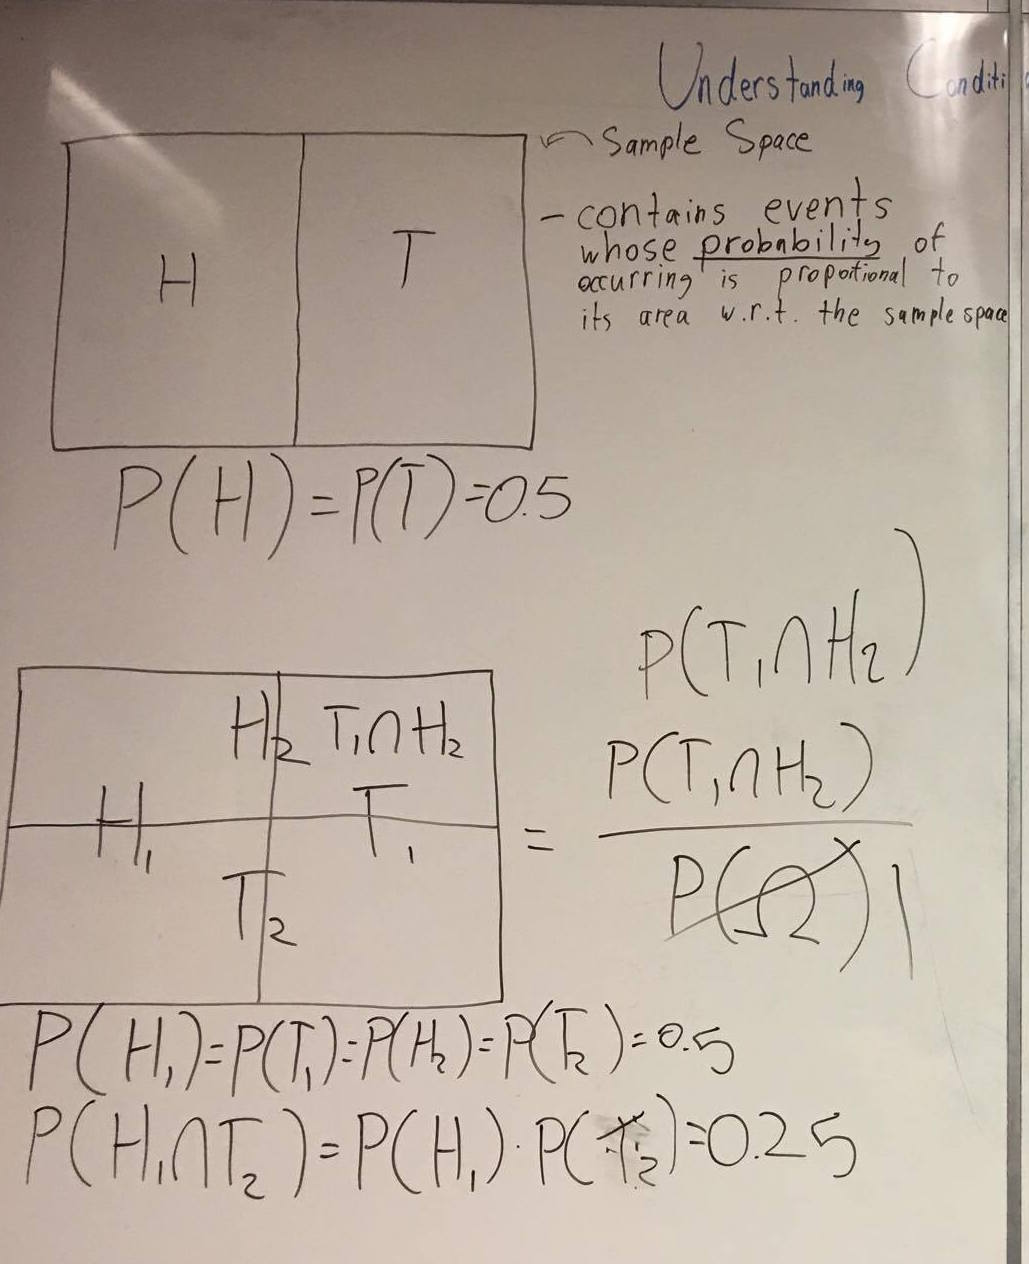
\includegraphics[width=.9\linewidth]{./img/conditional_probability_1.jpg}
\caption{\label{fig:orgparagraph1}
A visual representation of the sample space in the case of one and two coin flips.}
\end{figure}

\begin{figure}[htb]
\centering
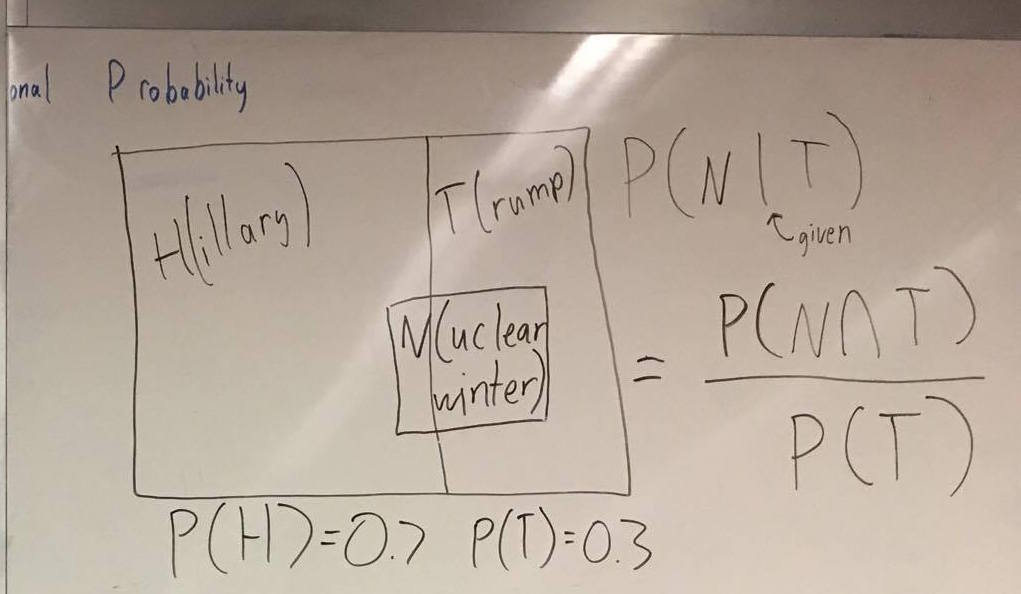
\includegraphics[width=.9\linewidth]{./img/conditional_probability_2.jpg}
\caption{\label{fig:orgparagraph2}
A visual representation of the sample space in conditional probability.}
\end{figure}

\begin{figure}[htb]
\centering
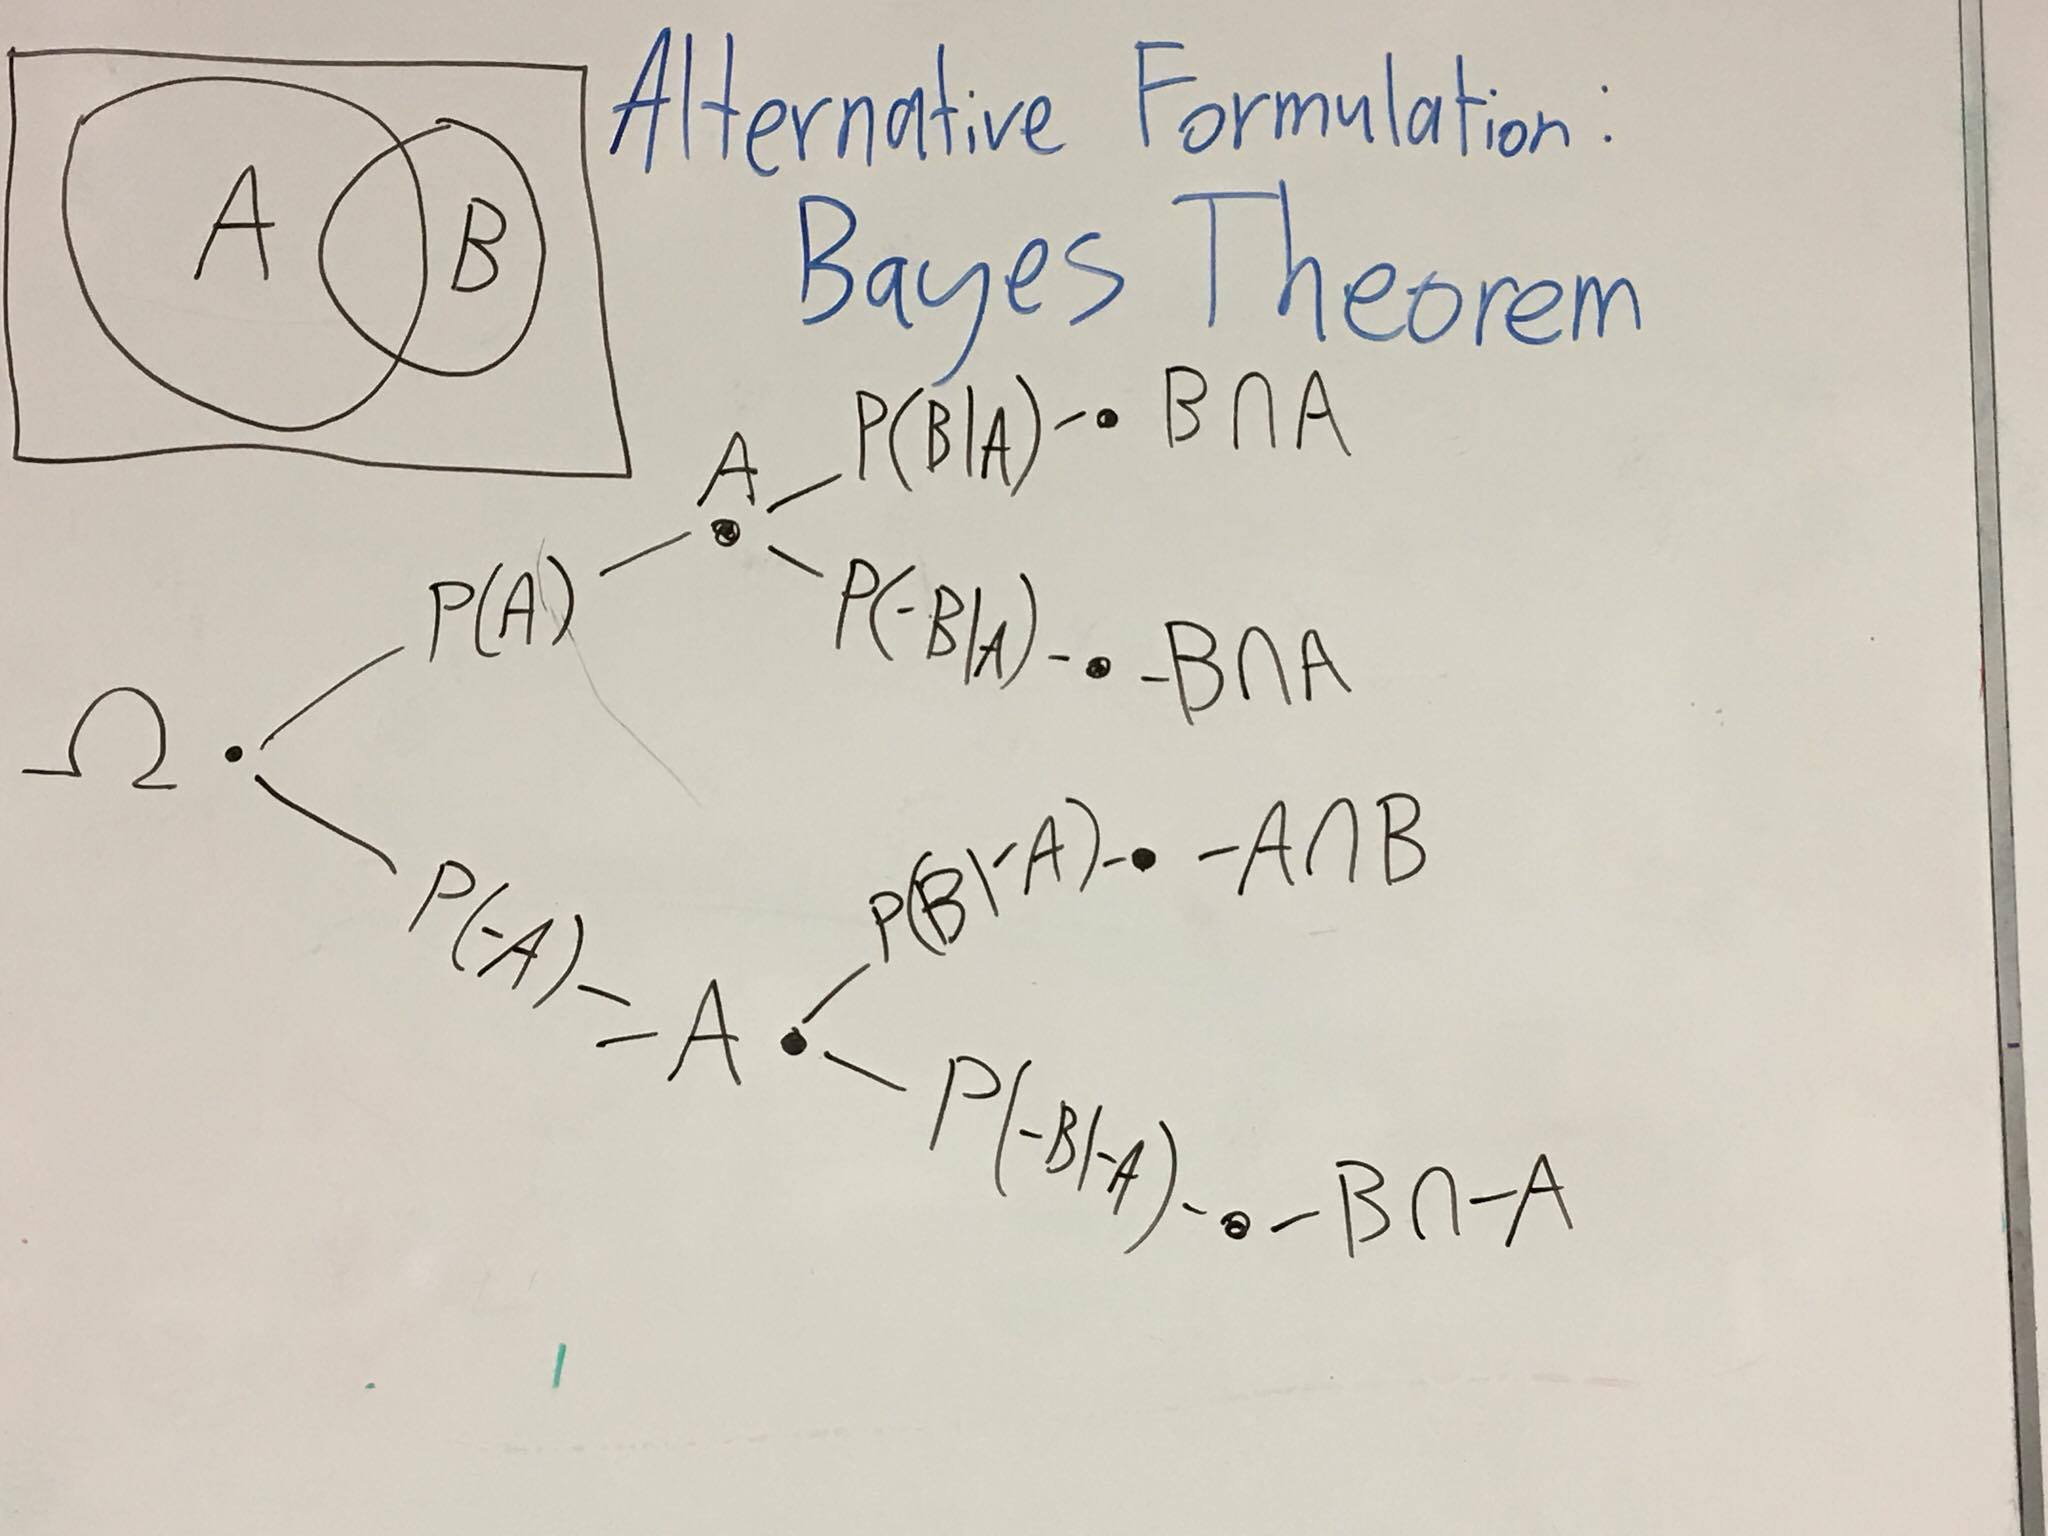
\includegraphics[width=.9\linewidth]{./img/bayes_tree.jpg}
\caption{\label{fig:orgparagraph3}
A visual representation of the sample space as conditional probabilities}
\end{figure}

\begin{figure}[htb]
\centering
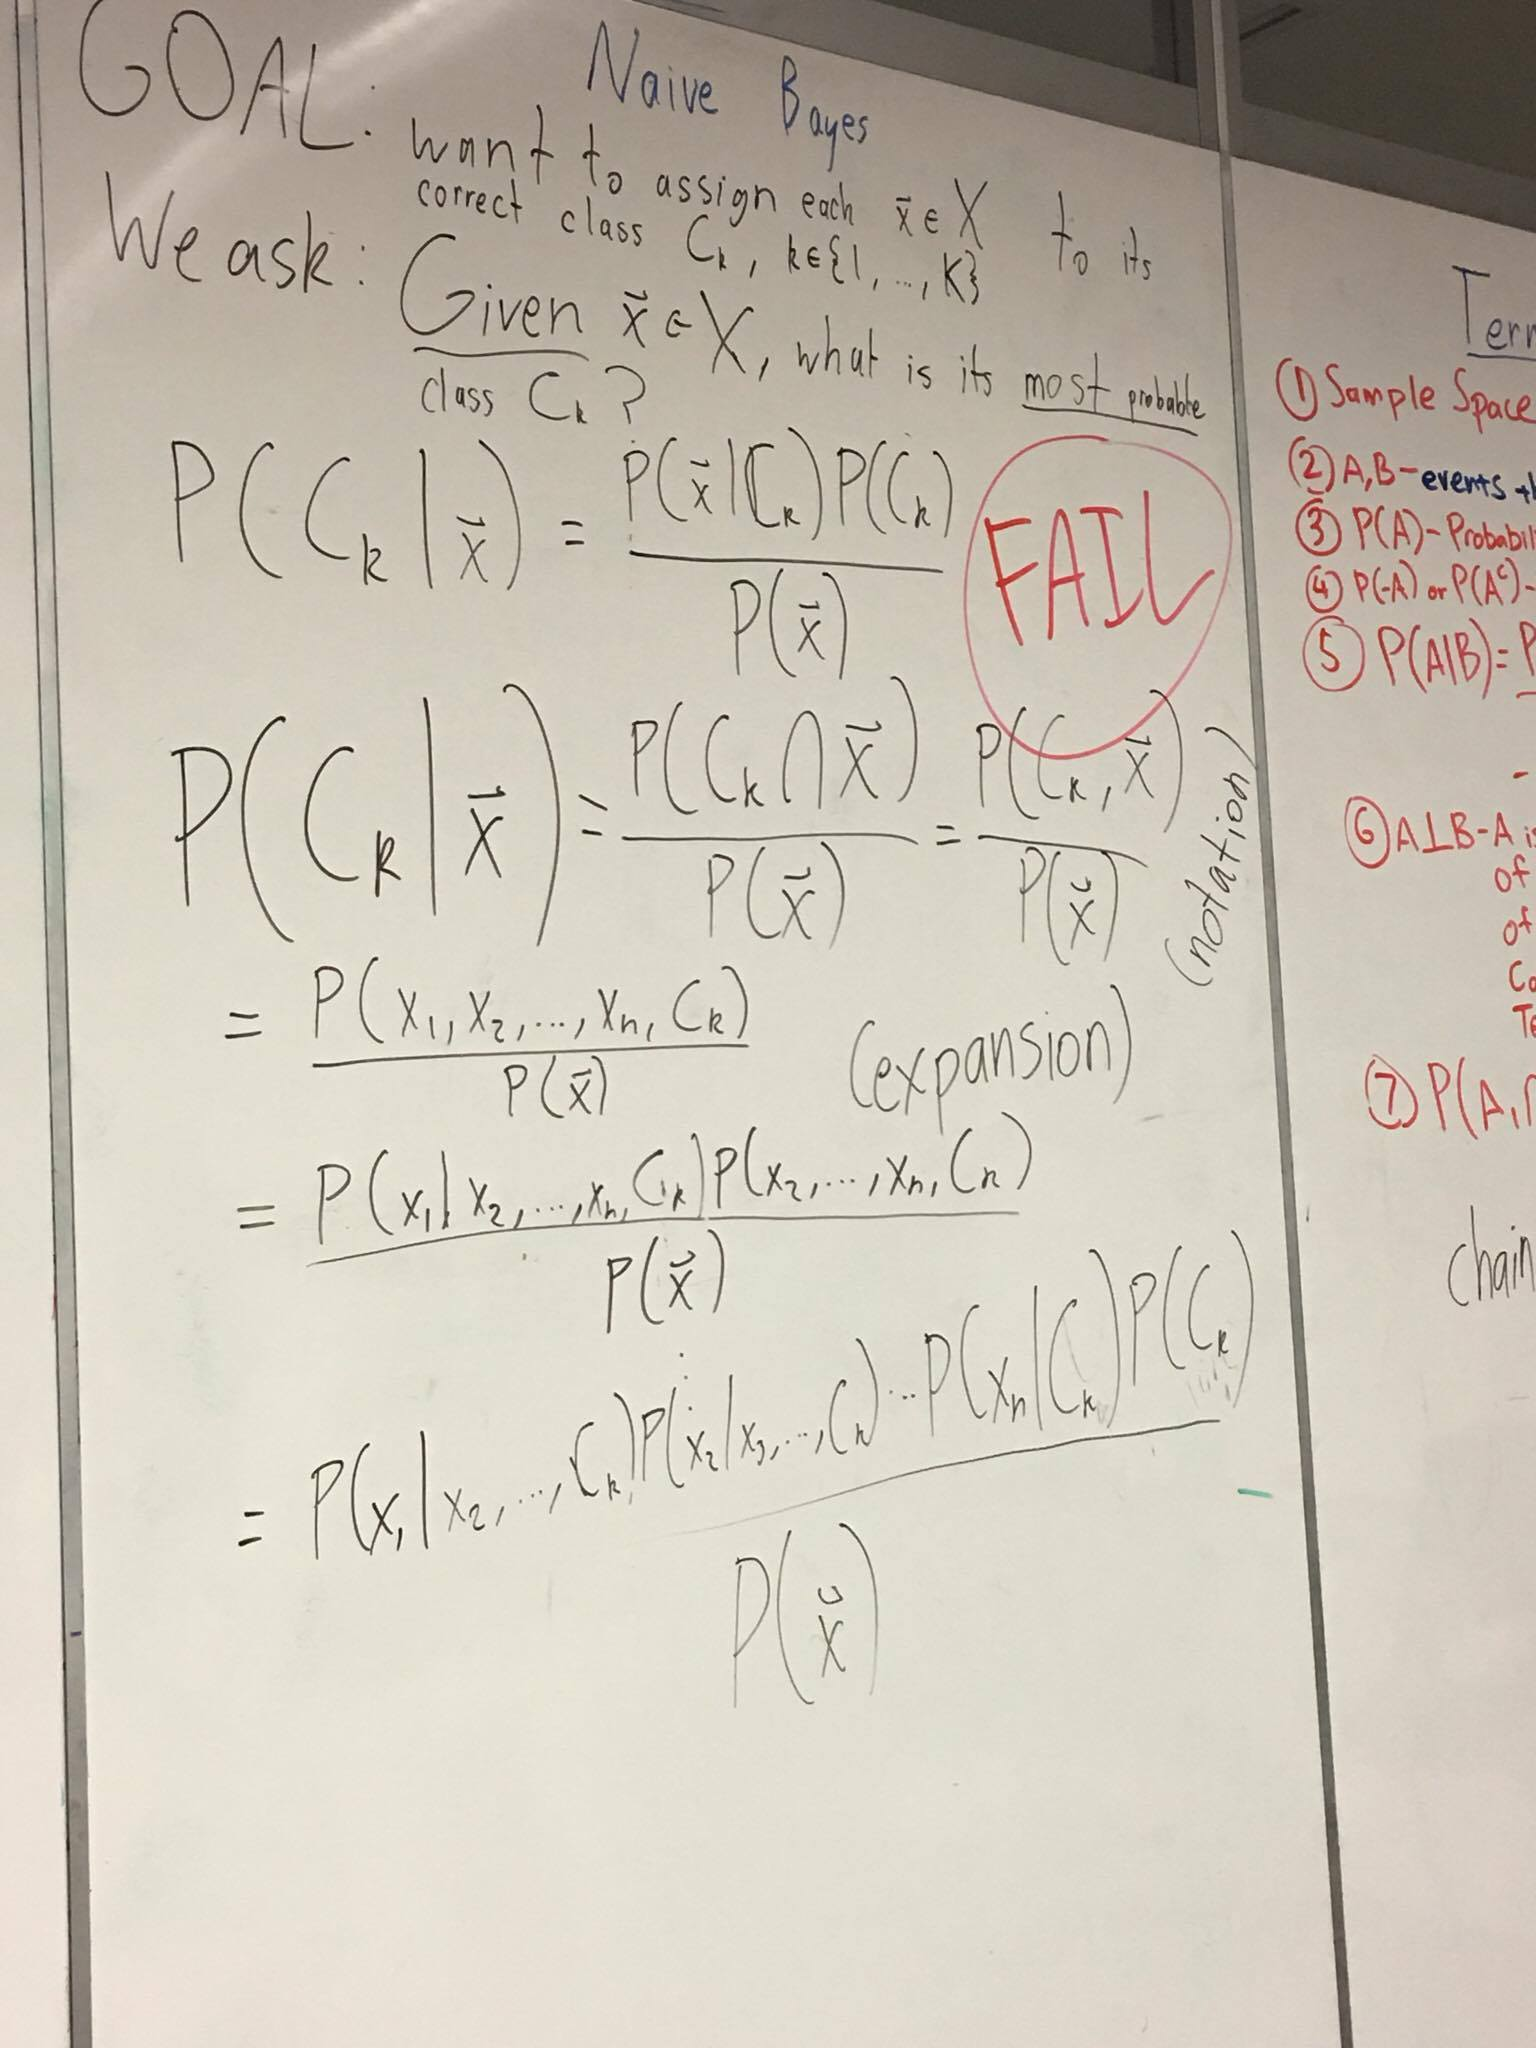
\includegraphics[width=.9\linewidth]{./img/naive_bayes.jpg}
\caption{\label{fig:orgparagraph4}
The expansion of bayes' theorem}
\end{figure}
\end{document}